\documentclass[10pt]{article}
\usepackage[letterpaper,margin=0.72in]{geometry}
\usepackage{times}
\usepackage{microtype}
\usepackage{graphicx}
\usepackage{booktabs}
\usepackage{xcolor}
\usepackage{hyperref}
\usepackage{enumitem}
\pagestyle{plain}
\hypersetup{colorlinks=true,linkcolor=black,urlcolor=blue}
\setlength{\parindent}{0pt}
\setlength{\parskip}{5pt}
\setlist[itemize]{leftmargin=1.2em,itemsep=2pt,topsep=2pt}
\definecolor{accent}{RGB}{37,94,142}
\definecolor{soft}{RGB}{244,248,251}
\newcommand{\boxnote}[1]{\colorbox{soft}{\parbox{\dimexpr\linewidth-2\fboxsep}{#1}}}
\begin{document}

\begin{center}
{\LARGE \textbf{Skill-Seam World/Action Models}}\\
{\large Four-page technical preview for collaboration outreach}\\[3pt]
\textcolor{accent}{\textbf{Predicting when composed robot skills will fail, diagnosing why, and choosing repair, abstain, or transition.}}
\end{center}

\section*{1. Problem: Composition Fails At The Handoff}

Independently competent robot skills can fail when chained. A module graph can mark skill $i\rightarrow j$ legal even when the terminal distribution of skill $i$ lies outside the attraction basin of skill $j$, crosses a high-energy barrier, or enters a contact mode where the next controller no longer descends. In those cases, the second skill is not merely ``hard to execute''; it is being asked to start from a physically invalid seam.

\boxnote{\textbf{Central question.} Can a robot predict whether a skill handoff is physically compatible before committing to the next behavior, then use the result to improve later plans?}

This project treats the handoff as a local world/action-modeling problem. The system estimates whether the next skill can take over, whether a small repair is enough, whether a diagnostic probe is needed, or whether the composition should abstain and choose another transition. The outcome becomes planner-edge evidence for future compositions.

\textbf{What this is not.}
\begin{itemize}
\item Not a new low-level impedance controller.
\item Not a universal robot policy.
\item Not a claim that local synthetic evidence is enough for deployment.
\item Not a request for a collaborator to supply the missing proof.
\end{itemize}

\textbf{What this is.}
\begin{itemize}
\item A local world/action model for skill seams.
\item A predictive representation of action consequences at skill boundaries.
\item A bounded energy-landscape mechanism for accept/repair/probe/abstain decisions.
\item A bridge toward adaptive physical world/action models for embodied agents.
\end{itemize}

\newpage
\section*{2. Method: Barrier-Certified Seam Scoring}

Let skill $i$ induce terminal distribution $p_i(x_T)$ and skill $j$ have attraction basin $\mathcal{B}_j$ under local controller $\pi_j$. A candidate handoff $h$ is accepted only when terminal samples overlap the next basin, barrier height is low enough, descent continuity remains positive, repair cost is acceptable, and calibrated seam risk is below a fixed-risk budget.

\[
S(i,j,h)=\alpha O_{\mathrm{basin}}(p_i,\mathcal{B}_j)-\beta B_{\mathrm{barrier}}(h,j)+\gamma D_{\mathrm{descent}}(h,j)-\lambda C_{\mathrm{repair}}(h)-\kappa R_{\mathrm{seam}}(h).
\]

\begin{center}
\begin{tabular}{ll}
\toprule
Term & Role at the seam \\
\midrule
$O_{\mathrm{basin}}$ & Does skill $i$ end inside skill $j$'s attraction region? \\
$B_{\mathrm{barrier}}$ & Does the transition cross a high-energy ridge? \\
$D_{\mathrm{descent}}$ & Does energy continue decreasing after handoff? \\
$C_{\mathrm{repair}}$ & How costly or unsafe is the repair? \\
$R_{\mathrm{seam}}$ & Is predicted risk below the fixed-risk budget? \\
\bottomrule
\end{tabular}
\end{center}

The composer chooses among:

\begin{itemize}
\item \textbf{Accept}: handoff is compatible under the fixed-risk budget.
\item \textbf{Repair}: small transition adjustment can recover the next basin.
\item \textbf{Probe}: information is insufficient; test the seam before committing.
\item \textbf{Abstain}: risk is too high or the energy model is miscalibrated.
\item \textbf{Fallback}: use another transition or ask for a new bridge skill.
\end{itemize}

\boxnote{\textbf{Bounded claim.} Energy-seam certification improves skill composition when basin overlap, barrier height, descent continuity, repair cost, and risk calibration are estimable. It must fail or abstain when primitives are broken, semantic goals conflict, or the landscape is invalid.}

\newpage
\section*{3. Current Local Evidence}

The current v5 local suite is frozen and reproducible. It tests 12 methods, 6 task families, 8 seam regimes, 5 deployment splits, 10 paired seeds, 230,400 main episode cells, 38,400 ablation cells, 161,280 stress cells, 107,520 fixed-risk cells, and 24 documented failure cases.

\begin{center}
\begin{tabular}{lcc}
\toprule
Hard-slice metric & Proposed composer & Strongest non-oracle predecessor \\
\midrule
Success & 0.80171 & 0.71711 \\
Utility & 0.88827 & 0.65310 \\
Paired utility wins & 10/10 & -- \\
Realized seam breach & 0.095 & 0.171 \\
\bottomrule
\end{tabular}
\end{center}

\begin{center}
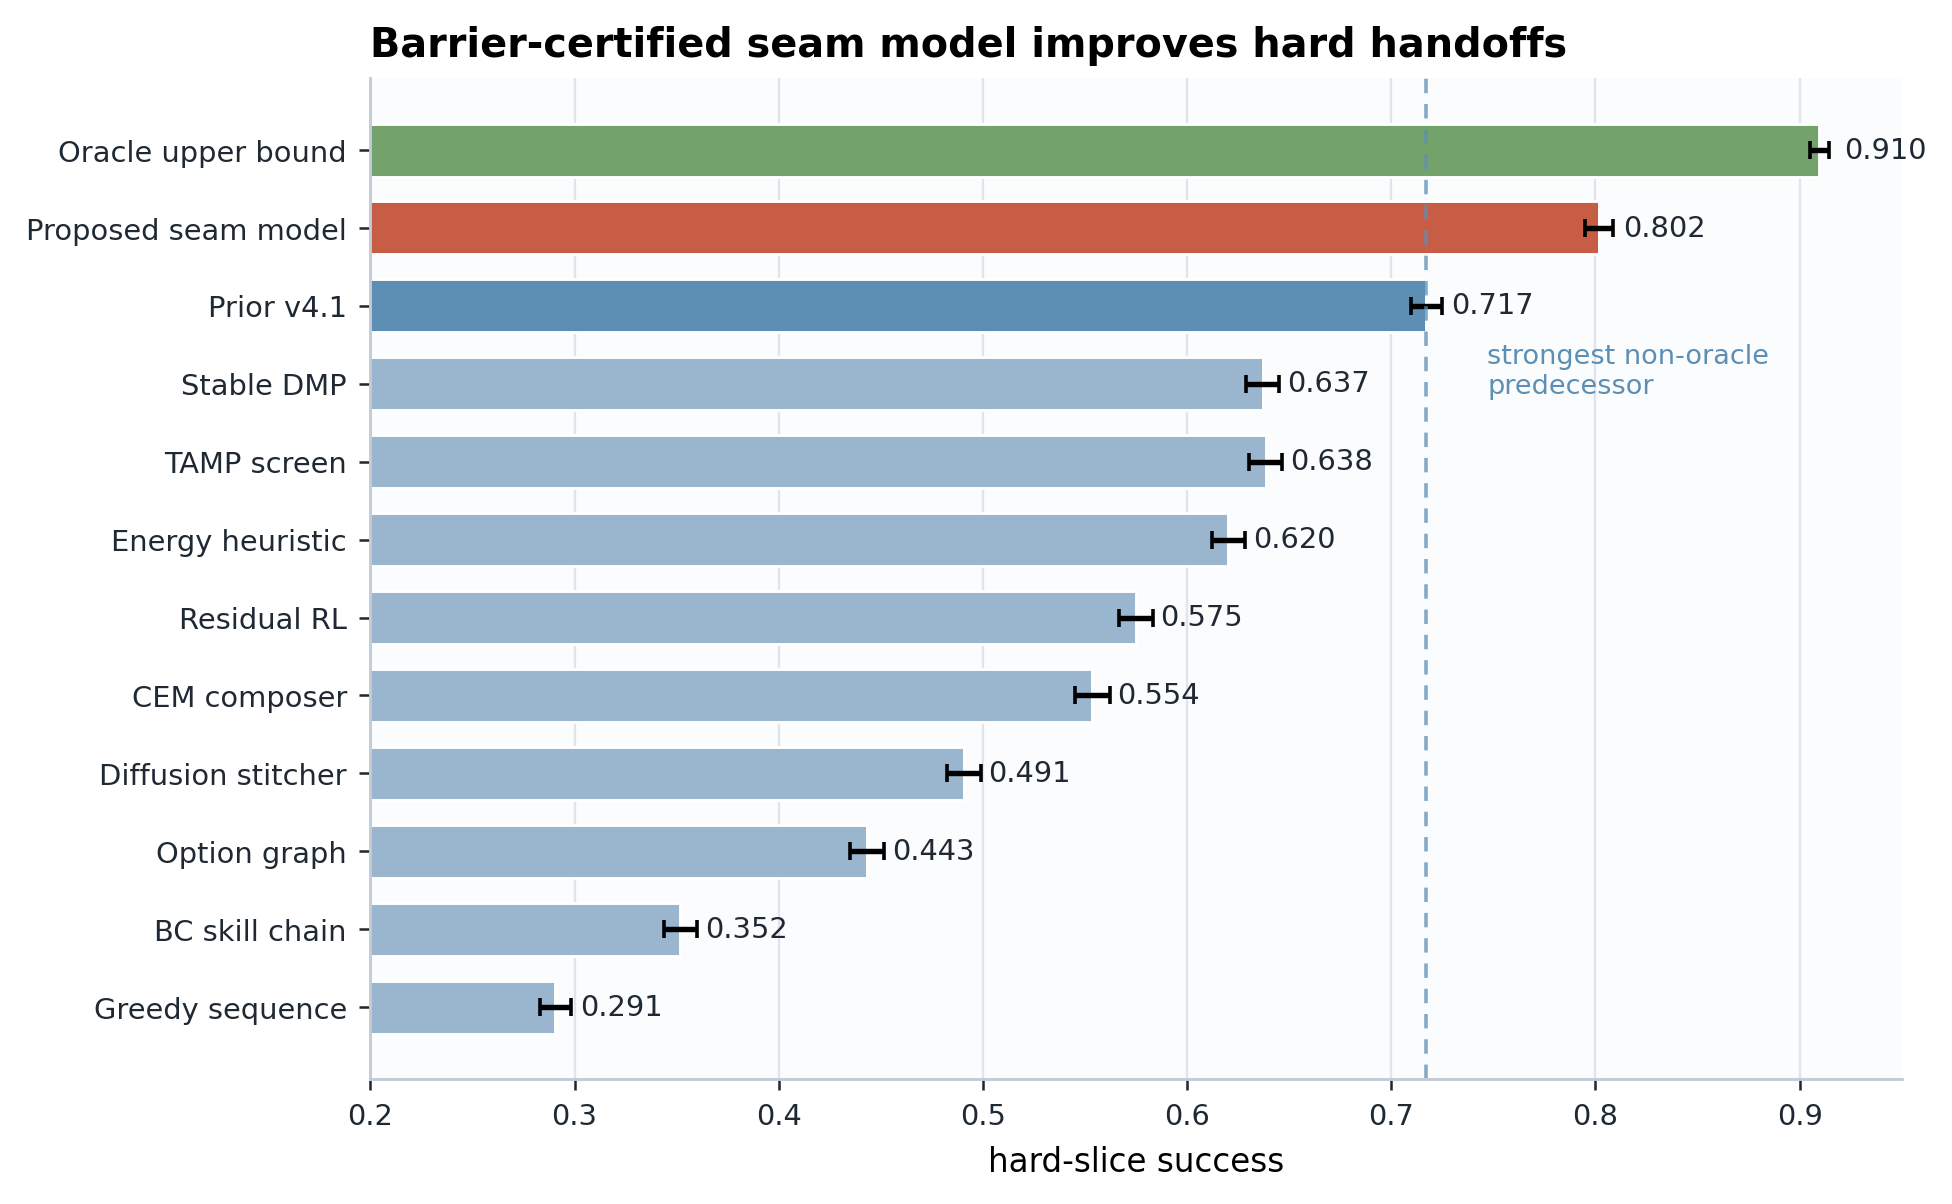
\includegraphics[width=0.86\linewidth]{../figures/energy_landscape_composition_hard_success_v5.png}
\end{center}

The proposed composer improves hard success by 0.08460 and hard utility by 0.23517 against the strongest non-oracle predecessor. It also reduces seam failure, barrier violation, damage, composition cost, risk calibration error, and realized seam breach while improving basin alignment and descent continuity. A diagnostic audit checks exported failure labels, seam decisions, and planner-edge updates over 230,400 local rows, so the mechanism evidence is not only aggregate success.

\textbf{Why this evidence is not enough yet.}
The current package is a strong local audit, not a final deployment claim. A main-conference version needs real robot or accepted high-fidelity skill-composition validation, released logs, videos, policy/checkpoint hashes, calibrated sensor/state traces, and manifest-declared independent baseline evidence from real external runs.

\newpage
\section*{4. Independent Validation And Collaboration Fit}

\textbf{Independent validation gate.}
Before the paper should be called independently submission-ready, it needs one of:
\begin{itemize}
\item at least 3 real robot composed tasks with paired resets;
\item at least 4 accepted high-fidelity simulation tasks with contact/dynamics fidelity;
\item a mixed route with 2 real robot tasks plus 2 high-fidelity simulation tasks.
\end{itemize}

Each run should use the same primitive skill library across baselines and log terminal samples, basin estimates, barrier scores, descent diagnostics, predicted risk, accepted/rejected seams, final outcomes, and videos. The repository has a generated operator packet that currently says \texttt{DO\_NOT\_COLLECT\_YET} until backend, real configs, fidelity acceptance, alias unsealing, and run identity pass strict gates.

\textbf{Why Haonan is the right first scientific contact.}
Haonan Chen's public research statement centers on multi-modal action composition: composing skills, action abstractions, and physics-inspired world models across sensory modalities and time scales. CoStream is especially relevant because it composes semantic, predictive, and reactive behaviors through a shared action interface.

\textbf{Why Yilun might care.}
Yilun Du's public research direction emphasizes generative models, decision making, robot learning, embodied agents, world models, planning, iterative reasoning, and composable energy landscapes. Paper 119 is naturally framed as a small predictive world/action model at the skill seam, not as low-level manipulation plumbing.

\textbf{Collaboration ask.}
The clean ask is not for a collaborator to validate the paper or supply the missing proof. The clean ask is:

\boxnote{Would a skill-seam world/action model be useful as a reliability layer in a CoStream-style behavior-composition stack, and what would be the cleanest falsification test?}

\textbf{Artifacts to send.}
\begin{itemize}
\item This four-page preview.
\item The one-page memo.
\item The independent validation protocol.
\item The operator packet if he asks how the external run would be gated.
\item A short email centered on CoStream, with at most one secondary pointer to SIMPACT or OAT.
\end{itemize}

\vfill
\textbf{Source anchors.}
\href{https://haonan16.github.io/}{Haonan Chen homepage};
\href{https://arxiv.org/abs/2606.26423}{CoStream};
\href{https://yilundu.github.io/}{Yilun Du homepage};
\href{https://arxiv.org/abs/2512.05955}{SIMPACT}.

\end{document}
